\subsection{Gas ideali}
Un gas ideale è costituito da particelle puntiformi, che non abbiano un proprio volume, e contenute in un recipiente cui è praticato il vuoto in modo da avere solo poche particelle del gase e dove abbiamo dei misuratori di temperatura e pressione.

Definiamo un gase "ideale" quando esso si trova a bassa pressione, quindi rarefatto e ad alta temperatura.

In queste condizioni è ragionevole assumere che non esistano interazioni fra le varie particelle, per cui esse si muovono in modo del tutto casuale. Qualora dovessero esserci urti, si assumono essere perfettamente elastici.

Un gas occupa l'intero volume che trova a sua disposizione ed esercita una pressione dovuta agli urti delle particelle del gas sulle superfici interne del recipiente che lo contiene.

Le proprietà di un gas sono determinate dalla sua pressione a la sua temperatura.

\vspace{0.2cm}La pressione, cioè la forza esercitata sulle pareti, ha come unità di misura l'\textit{atmosfera (atm)}. Inoltre $1 \; atm=760 \; mmHg=1 \; Torr$. Nel S.I. l'unità di misura è il \textit{Pascal (Pa)}, per cui

$$P=N/m^2=\big[ (kg \cdot m)/s^2 \big]/m^2=(kg \cdot m)(s^2 \cdot m^2)$$
$$\rightarrow P=kg/(s^2 \cdot m)$$

Spesso nelle bombole l'unità di misura è il \textit{bar}. 1 bar equivale a $10^5 \; Pa$.

LA temperatura si misura in gradi centigradi (°C) o in gradi Kelvin (K).
\subsection{Significato molecolare della pressione}
La pressione è dovuta agli urti delle particelle contro le pareti del recipiente che lo contiene ed è la stessa in tutti i suoi punti.
\subsection{Significato molecolare della temperatura}
Supponiamo di avere un gas dentro un contenitore chiuso e di riscaldarlo mantenendo costante il suo volue. Ci accorgiamo che aumenta la pressione, cioè aumenta il numero di urti delle particelle nell'unità di tempo. Se aumentano gli urti, aumenterà la velocità delle particelle. Dalla teoria cinetica molecolare sappiamo che l'energia cinetica di una particella è pari a $E_k=3/2 K_bT$, dove $K_b$ è la costante di Boltzmann e $T$ è la temperatura.

\hspace{0.5cm}\begin{minipage}{0.55 \textwidth}
    \begin{figure}[H]
        \includegraphics[width=8cm]{immagini/velocità_molecolare.png}
    \end{figure}
\end{minipage}
\begin{minipage}{0.4 \textwidth}
Consideriamo l'O$_2$. Notiamo che a 25° C la porzione di molecole che ha velocità elevata è ristretta, mentre a 1000° C tale porzione è molto maggiore.

Deduciamo che aumentare la temperatura significa aumentare la velocità media della maggior parte delle particelle e aumentare la porzione di particelle che hanno velocità molto elevate.
\end{minipage}

\subsection{Legge di Boyle}
Se manteniamo costante la temperatura (trasformazione isoterma), il prodotto $P \cdot V$ è costante.

Se quindi il gas subisce $n$ trasformazioni isoterme varrà

$$P_0V_0=P_1V_1=P_2V_2=...=P_nV_n$$

con $P_0$ e $V_0$ condizioni iniziali del gas.


\begin{figure}[htp]
    \centering
    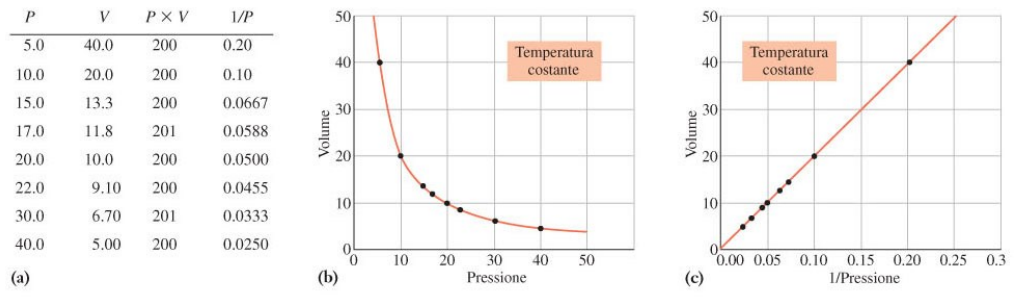
\includegraphics[width=16cm]{immagini/Legge_di_Boyle.png}
\end{figure}

La legge può essere espressa come

$$PV=k \qquad P=\frac{k}{V} \qquad V=\frac{k}{P}$$

o, in forma logaritmica, come $logV = logk - log P$
\subsection{Legge di Charles (Gay-Lussac)}
\subsection{Legge di Gay-Lussac}
\subsection{Legge di Dalton e delle pressioni parziali}
\subsection{Legge dei volumi molare e di Avogadro}
\subsection{Equazione di stato}
\subsection{Determinazione dei pesi molecolari}
\subsection{Gas e vapori}